%	현대물리실험 보고서
%	실험1
%	202100973 이승엽

%----------------------------------------------------------------------------------------
%	PACKAGES AND DOCUMENT CONFIGURATIONS
%----------------------------------------------------------------------------------------

\documentclass[a4paper, 10pt, nanum]{CSUniSchoolLabReport}
% use UTF8 encoding
\usepackage[utf8]{inputenc}
% use KoTeX package for Korean
\usepackage{kotex}
\usepackage{amsmath}
\usepackage{hyperref}
\usepackage{graphicx}
\usepackage{indentfirst}
\usepackage{setspace}
\usepackage{multirow}
\usepackage{enumitem}
\usepackage{graphicx}
\usepackage{wrapfig}
\usepackage{epstopdf}

\setlength{\parindent}{0.2in} % 들여쓰기 길이 설정
\setlength{\parskip}{3mm} % 문단 간의 간격 조절
\setstretch{1.5} % 줄간격

\addbibresource{reference.bib} % Bibliography file (located in the same folder as the template)

%----------------------------------------------------------------------------------------
%	REPORT INFORMATION
%----------------------------------------------------------------------------------------

\title{현대물리실험 실험1 보고서 \\ Energy loss of Alpha-particles in gases with MCA} % Report title

\author{\textsc{Department of Physics} 202100973 이승엽}

\date{\today}

%----------------------------------------------------------------------------------------

\begin{document}

\maketitle % Insert the title, author and date using the information specified above

\begin{center}
	\begin{tabular}{l r}
		Date Performed: & March 28, 2023 \\ % Date the experiment was performed
		& April 4, 2023 \\
		Partners: & 202100969 이규리 \\ % Partner names
		& 202100989 한누리 \\
		Instructor: & Professor 이기주 \\ % Instructor/supervisor
		Typesetting: & LaTeX \\
		Data Fitting: & OriginPro
	\end{tabular}
\end{center}

%----------------------------------------------------------------------------------------
%	ABSTRACT
%----------------------------------------------------------------------------------------

\maketitle
% \begin{abstract}
% 	This report ...
% \end{abstract}

%----------------------------------------------------------------------------------------
%	INTRODUCTION
%----------------------------------------------------------------------------------------

\section{서론}

	The energy sensitivity of the detector is calibrated with an uncovered $^{241}\textrm{AM}$-source in vacuum. The dependence of the energy loss of $\alpha$-particles on the concentration of air particles between source and detector is measured. The dependence of energy loss of the $\alpha$-particles on the sort of gas particles between source and detector is determined and compared to the electron density in that sort of gas.

	\begin{enumerate}[label=\arabic*.]
		\item The	pulse	height	spectrum	resulting	from	 $\alpha$-particles	coming	from	an	uncovered		 	$^{241}\textrm{AM}$ emitter	is	recorded	with	the
		MCA.	The	 -particle	energy	of	the	principal	peak,	5,468 MeV,	is	used	for	calibration.
		\item The	spectrum	of	 $\alpha$-particles	reaching	the	detector	from	a	covered	 $^{241}\textrm{AM}$	source	in	10 cm 	distance	from	the	detector	is
		recorded	in	dependence	on	air	pressure.	The	rate	of	energy	loss	in	dependence	on	particle	energy	is	evaluated	and
		compared	to	predictions	by	the	Bethe-formula.
		\item The	spectrum	of	$\alpha$ -particles	reaching	the	detector	from	a	source	at	10 cm 	distance	in	helium,	carbon	dioxide	and	nitrogen
		with	100 hPa 	pressure	is	recorded.	The	energy	loss	in	dependence	on	electron	density	is	compared	to	predictions	by	the
		Bethe-formula.
	\end{enumerate}

%----------------------------------------------------------------------------------------
%	THEORY
%----------------------------------------------------------------------------------------

\section{이론}

	$\alpha$-decay 처럼 무거운 핵은 에너지 적으로 4He 핵을 비교적 쉽게 방출된다. 예를 들어 하나의 $^{241}\textrm{AM}$ 원자의 결합 에너지는 52.9360 MeV이고, 하나의 237Np 원자의 결합 에너지는 44.8733 MeV이다. 또한 4He 원자는 2.4249 MeV의 결합에너지(binding energy)를 갖는다. 결국 $^{241}\textrm{AM}$의 $\alpha$-decay에서 5.6378 MeV 만큼의 양이 알파 붕괴를 위해 사용 가능하다.

	반응 시 운동량은 $\alpha$-particle과 반동에 의해 방출된 nucleus이 균등하게 분리된다. 이것으로부터 에너지는 질량의 비율이 반응 생성물의 에너지의 비율과 같아지도록 분리되며 다음의 수식을 따른다,
	\begin{align*}
		(E_1 + E_2) = E_1 \left( 1 + \frac{4}{237} \right) = 5.6378 ~\textrm{MeV}
	\end{align*}

	방출한 핵이 excited state에 있다면, the excitation energy가 the $\alpha$-particle의 운동에너지로 사용될 수 없다. excitation(여기상태)는 떠나는 핵과 반동된 핵을 형성하기 위한 nucleons(핵자)의 배열에 몇 가지 가능한 효과로 생각 할 수 있다. 남겨진 nucleons는 다른 구성으로 존재할 수 있고, $\gamma$-decay에 의해 가장 낮은 에너지의 구성에 도달하기 위해 재정렬 될 수도 있다. 

	$^{241}\textrm{AM}$의 경우에는, 몇 가지 가능한 nuclear states가 있으며 그 가능한 nuclear states에 방출된 핵이 남겨진다. 따라서 $\alpha$-particles는 최대운동에너지에서 특정 excited nuclear state의 에너지를 뺀 에너지로 발생된다. 알파 에너지 스펙트럼은 방출로 인한 핵이 안정적으로 배열되도록 몇몇 에너지띠를 가지고 있다.

	실재로는 $\alpha$-particles의 최대에너지와 실제 에너지 차이만큼의 photons이 존재한다. 하지만 이 실험에서는 광자가 기록되지 않는다. 이러한 광자는 우리가 사용하는 detector에 상호작용하지 않고 감지되지 않는다.

%----------------------------------------------------------------------------------------
%	EXPERIMENTAL METHOD
%----------------------------------------------------------------------------------------

\section{실험 방법}

	\begin{figure}[htb!]
		\centering
		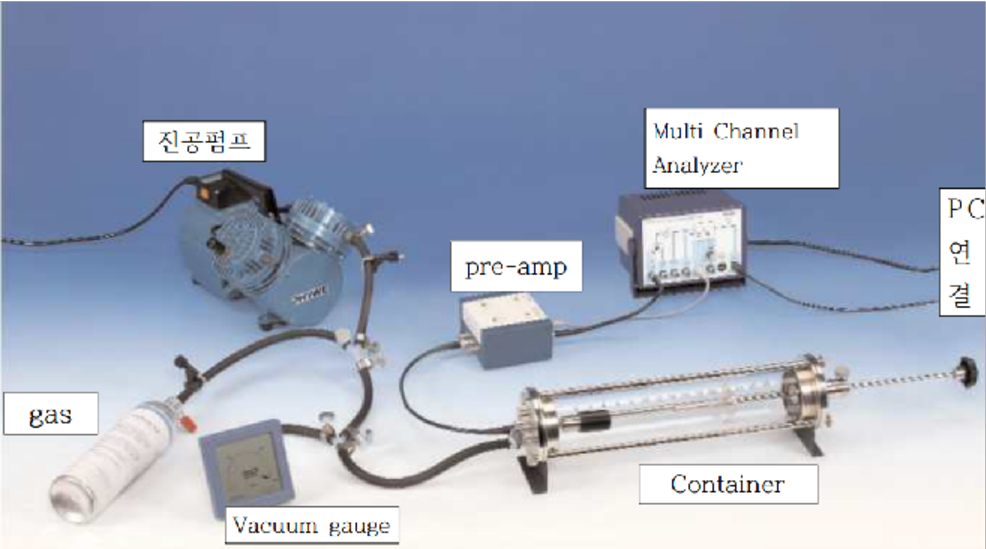
\includegraphics[width=8cm]{fig1.pdf}
		\caption{장비가 연결되어 있는 모습}
		\label{fig:1}
	\end{figure}

\subsection{실험 장비 셋업}

	실험세팅이 되어있다. 처음에는 gas가 없는 상태로 있는 bottle이 미세조정벨브와 핀치코크에 연결되어 있다. Background 스펙트럼은 관의 구멍을 다 열고 측정할 수 있다. Background 스펙트럼을 측정시에는 빛을 조심한다. light detector 이기 때문에 빛이 들어가지 않도록 덮는 게 좋다. 검은 쉴딩이 detector을 덮고 있고 detector는 flange cover에 닿아 있다. 3.7 kBq의 아메리슘 소스를 까만색 detector에 넣고 빛을 차광한다. 너무 깊게 넣어 detector에 닿지 않도록 주의한다. Pre-amplifier 스위치는 알파로 setting하고 Inv.로 둔다. 처음실험에서는 gas를 연결하지 않고 진공상태에서만 진행하며 진공펌프 가동이전에 컨테이너를 공기가 삽입되지 않도록 주의하며 방사능소스를 삽입한다. (맨 처음 실험 시 설명.)

\subsection{pc와 Multi Channel Analyzer(Cobra3)을 연결.}

	방사능 소스에서 나오는 에너지는 컨테이너 맨 끝에 위치한 detector를 지나서 Pre-amplifier를 지나서 데이터 처리기인 Multi Channel Analyzer(Cobra3)를 지나 신호를 처리하여 PC로 연결된다. PC에서 ‘measure’단추를 찾아 프로그램을 실행 시킨 후 시행한다. 

\subsection{그래프 및 수치화된 데이터를 날짜, 거리, gas등으로 하여 저장.}

	에너지와 에너지 손실값을 계산한다.

%----------------------------------------------------------------------------------------
%	RESULT AND DISCUSSION
%----------------------------------------------------------------------------------------

\section{실험 결과 및 해석}

%----------------------------------------------------------------------------------------
%	EXPERIMENTAL DATA AND ANALYSIS
%----------------------------------------------------------------------------------------

\subsection{실험 데이터}

	실험 데이터는 Channel 수(event)를 계속 만들어내고, 그에 따른 중첩된 Intensity를 측정한 것이다. 이때, Channel이 클수록(event가 많을수록) 데이터가 많이 검출되었다는 의미이므로, 데이터 peak의 x-axis는 큰 의미에서 데이터 검출량으로 봐도 무방하다.

	데이터는 measure 프로그램을 사용하여 smooth fitting한 것이며, 이 데이터를 OriginPro에서 Gaussian fitting하여 peak point를 찾아내었다.

	\begin{figure}[htb!]
		\centering
		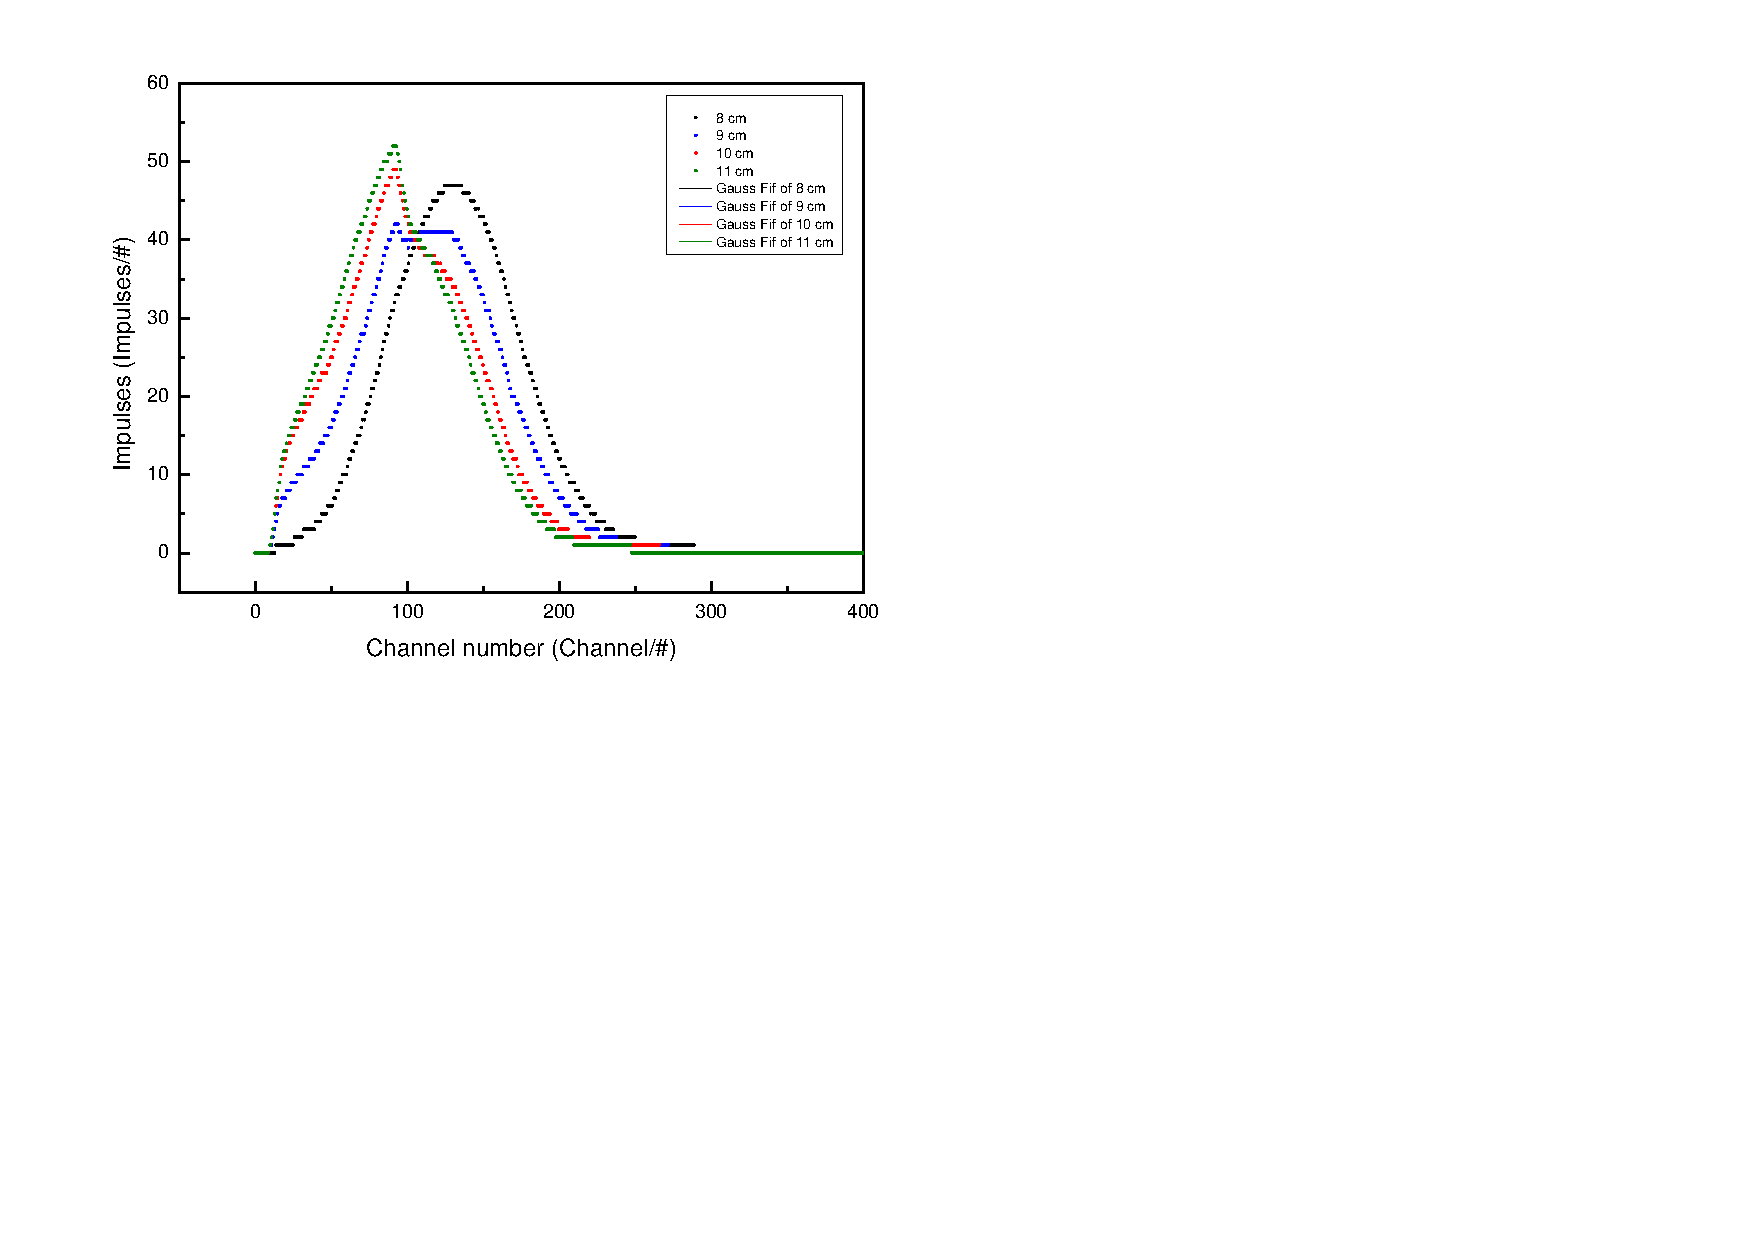
\includegraphics[viewport=1mm 99mm 180mm 200mm, width=9cm, clip=true]{fig2.pdf}
		\caption{거리에 따른 에너지 손실 그래프이다.}
		\label{fig:2}
	\end{figure}

	\begin{figure}[htb!]
		\centering
		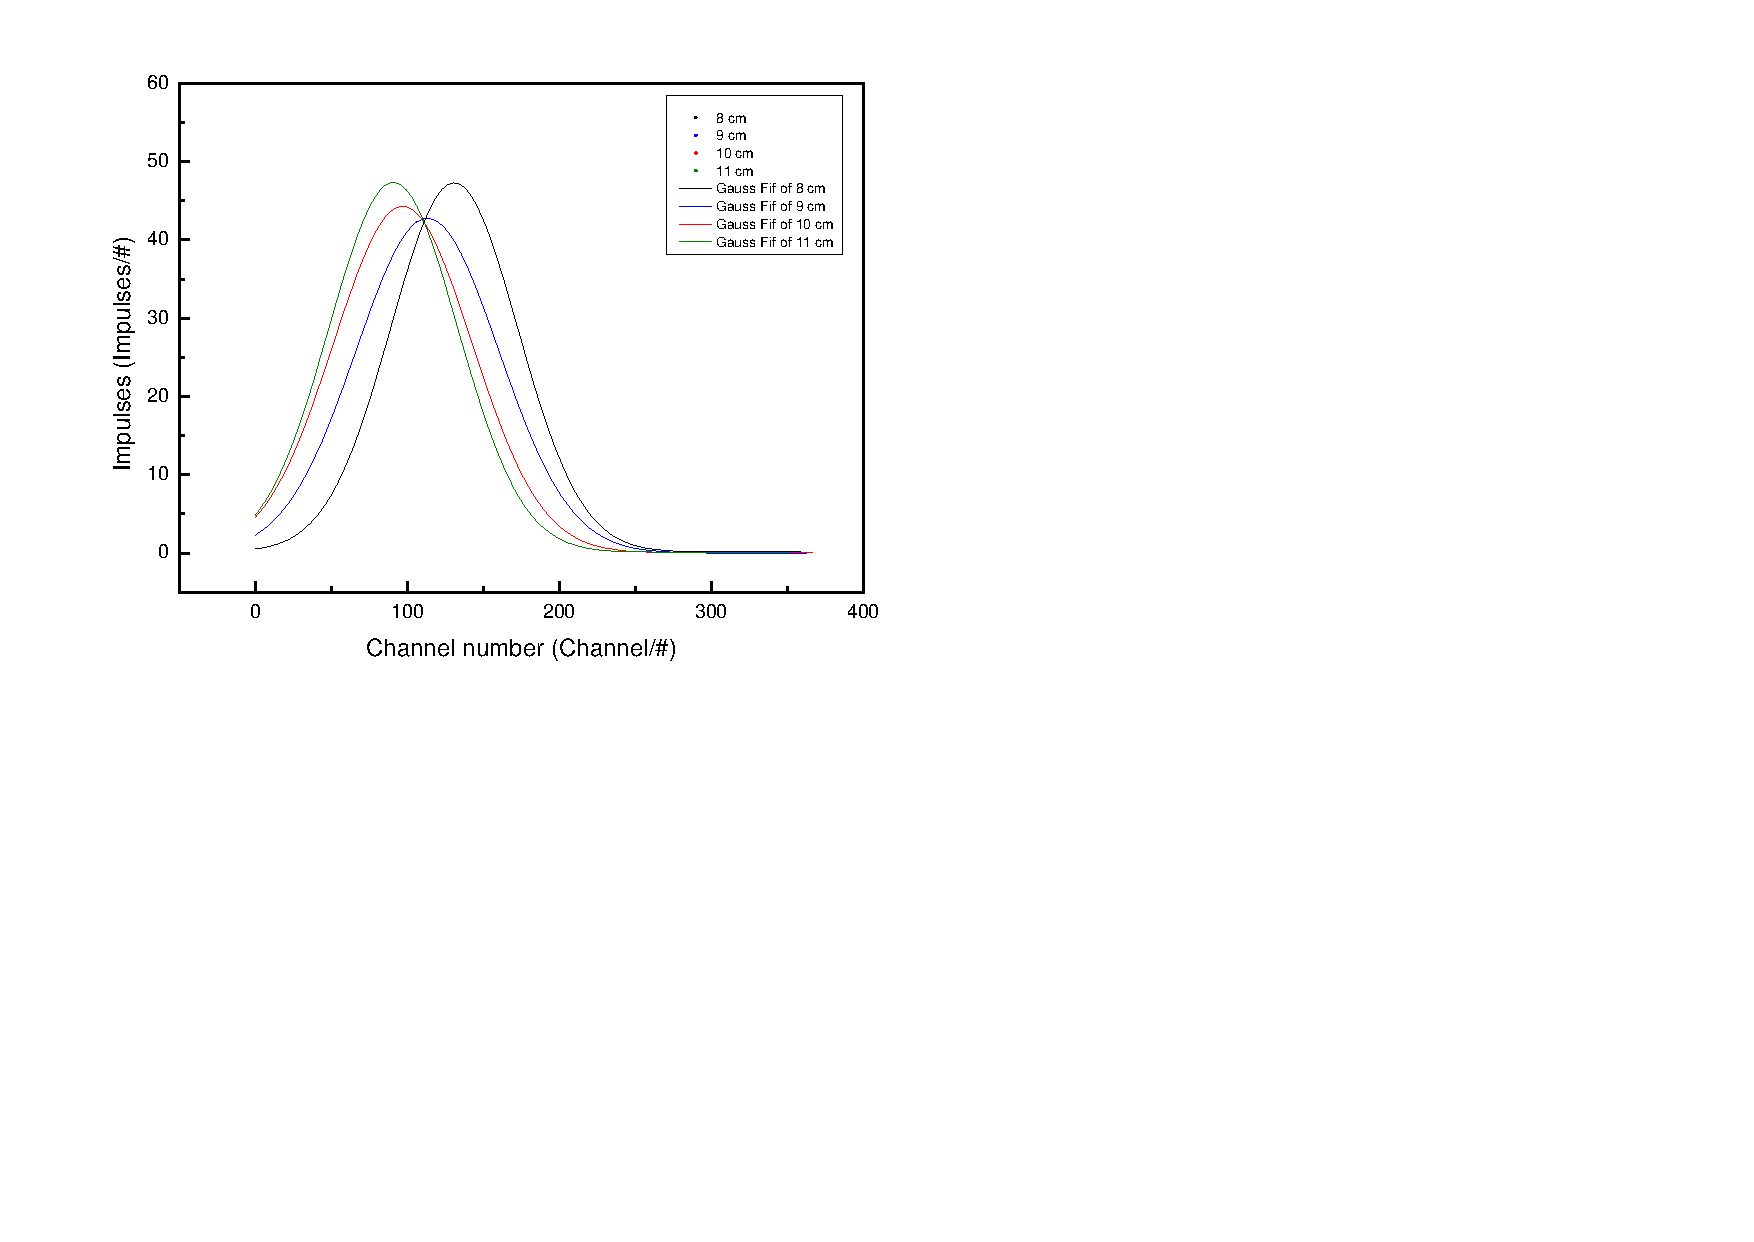
\includegraphics[viewport=1mm 99mm 180mm 200mm, width=9cm, clip=true]{fig3.pdf}
		\caption{거리에 따른 에너지 손실 그래프를 가우시안 함수로 피팅한 것이다.}
		\label{fig:3}
	\end{figure}

	(Fig. 3)에서 검정색 데이터는 8 cm, 파란색은 9cm, 빨간색은 10 cm, 초록색은 11 cm이다. 해석하면 데이터의 Peak의 Channel 값, 즉 검출량이 거리가 멀어질수록 적어짐을 볼 수 있고, 또한 Intensity가 커짐을 볼 수 있다. 8 cm에서 Intensity가 큰 이유는 event 수를 2배 늘려 실험을 진행했기 때문에, 이러한 경향을 보인다.

	\begin{table}[htb!]
		\label{tab:1}
		\centering
		\caption{거리에 따른 에너지 손실에 관한 표이다.}
		\begin{tabular}{c|cccc}
			\noalign{\smallskip}\noalign{\smallskip}\hline\hline
			\multirow{2}{*}{Data} &  \multicolumn{4}{c}{Distance} \\
			\cline{2-5}
				& 8 cm & 9 cm & 10 cm & 11 cm \\
			\hline
				Channel No. & 131.06 & 113.48 & 97.28 & 91.08 \\
				Peak Intensity & 47.19 & 42.80 & 44.32 & 47.28 \\
			\hline
			\hline
		\end{tabular}
	\end{table}


	\begin{figure}[htb!]
		\centering
		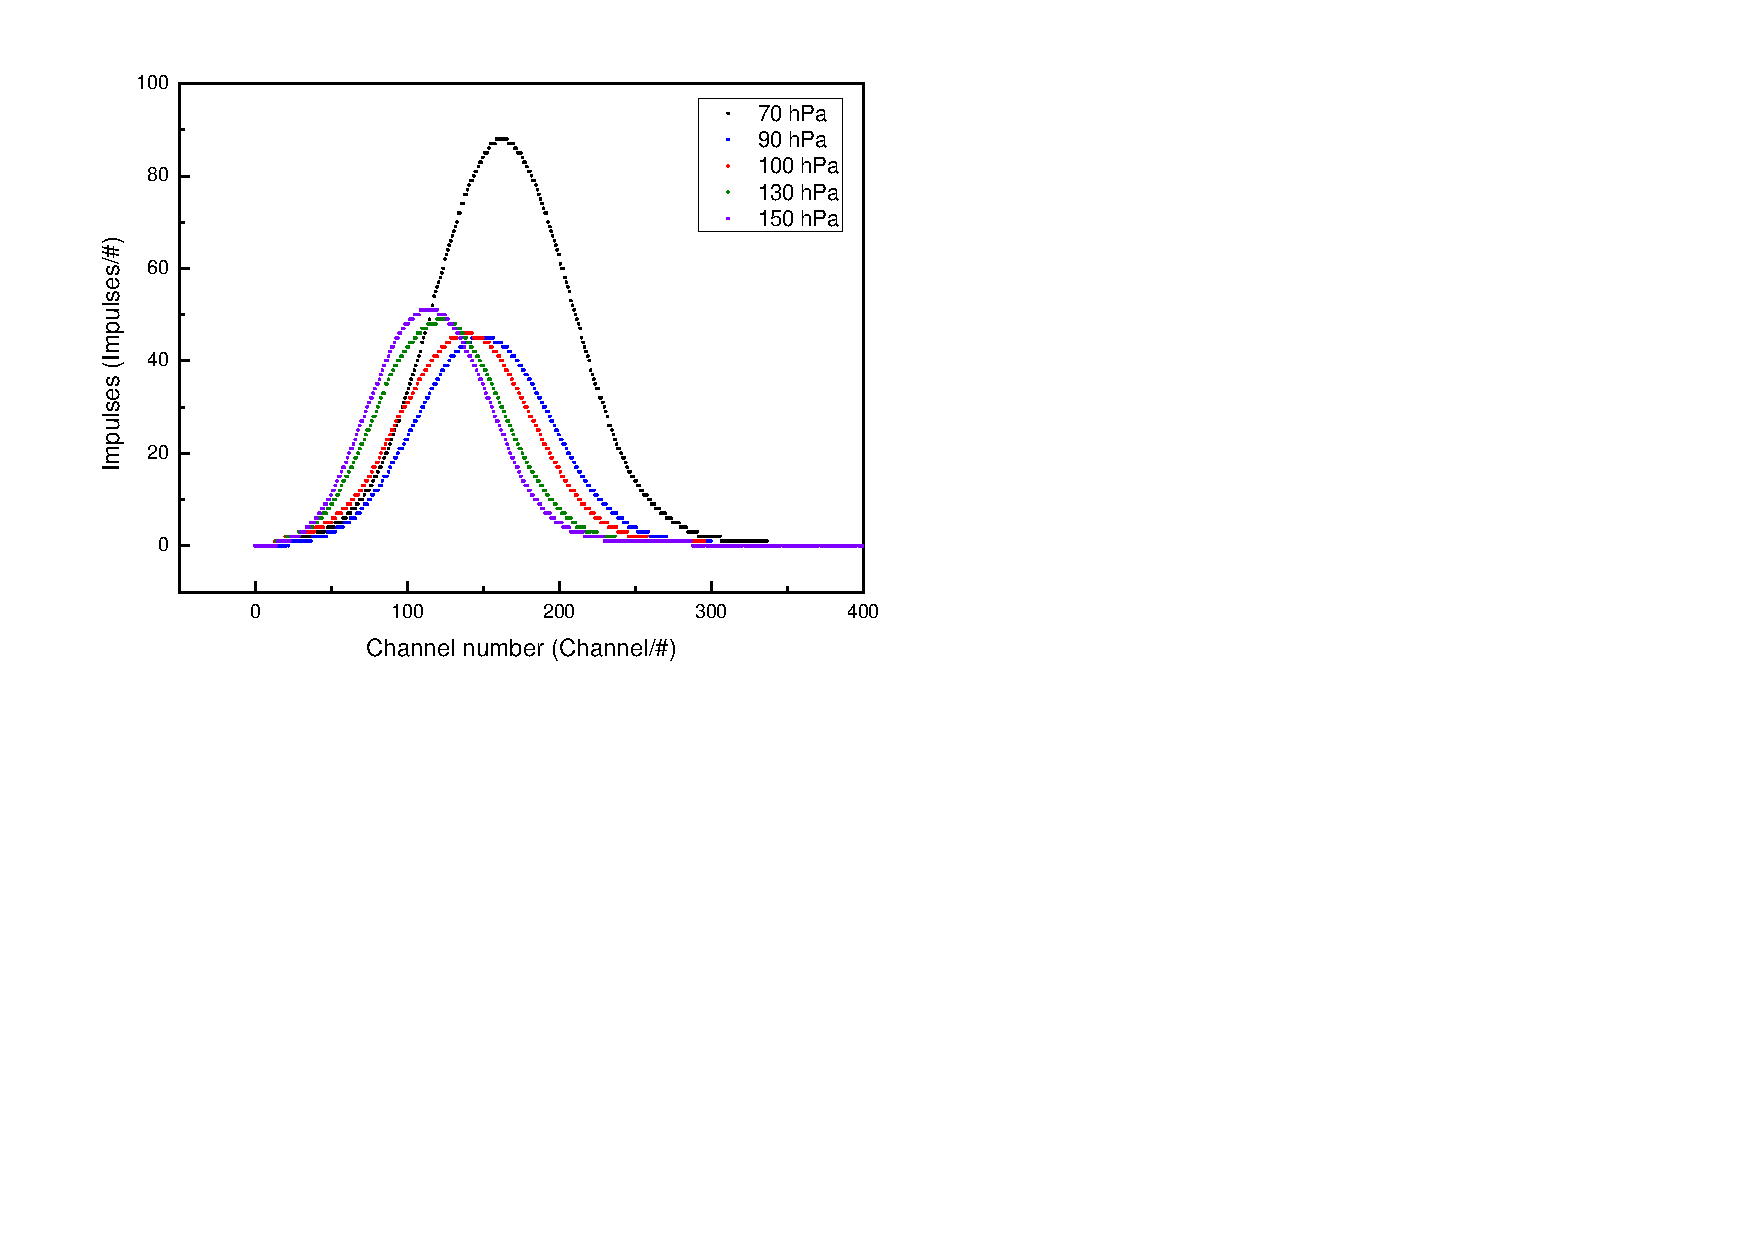
\includegraphics[viewport=1mm 99mm 180mm 200mm, width=9cm, clip=true]{fig4.pdf}
		\caption{압력에 따른 에너지 손실 그래프이다.}
		\label{fig:4}
	\end{figure}

	\begin{figure}[htb!]
		\centering
		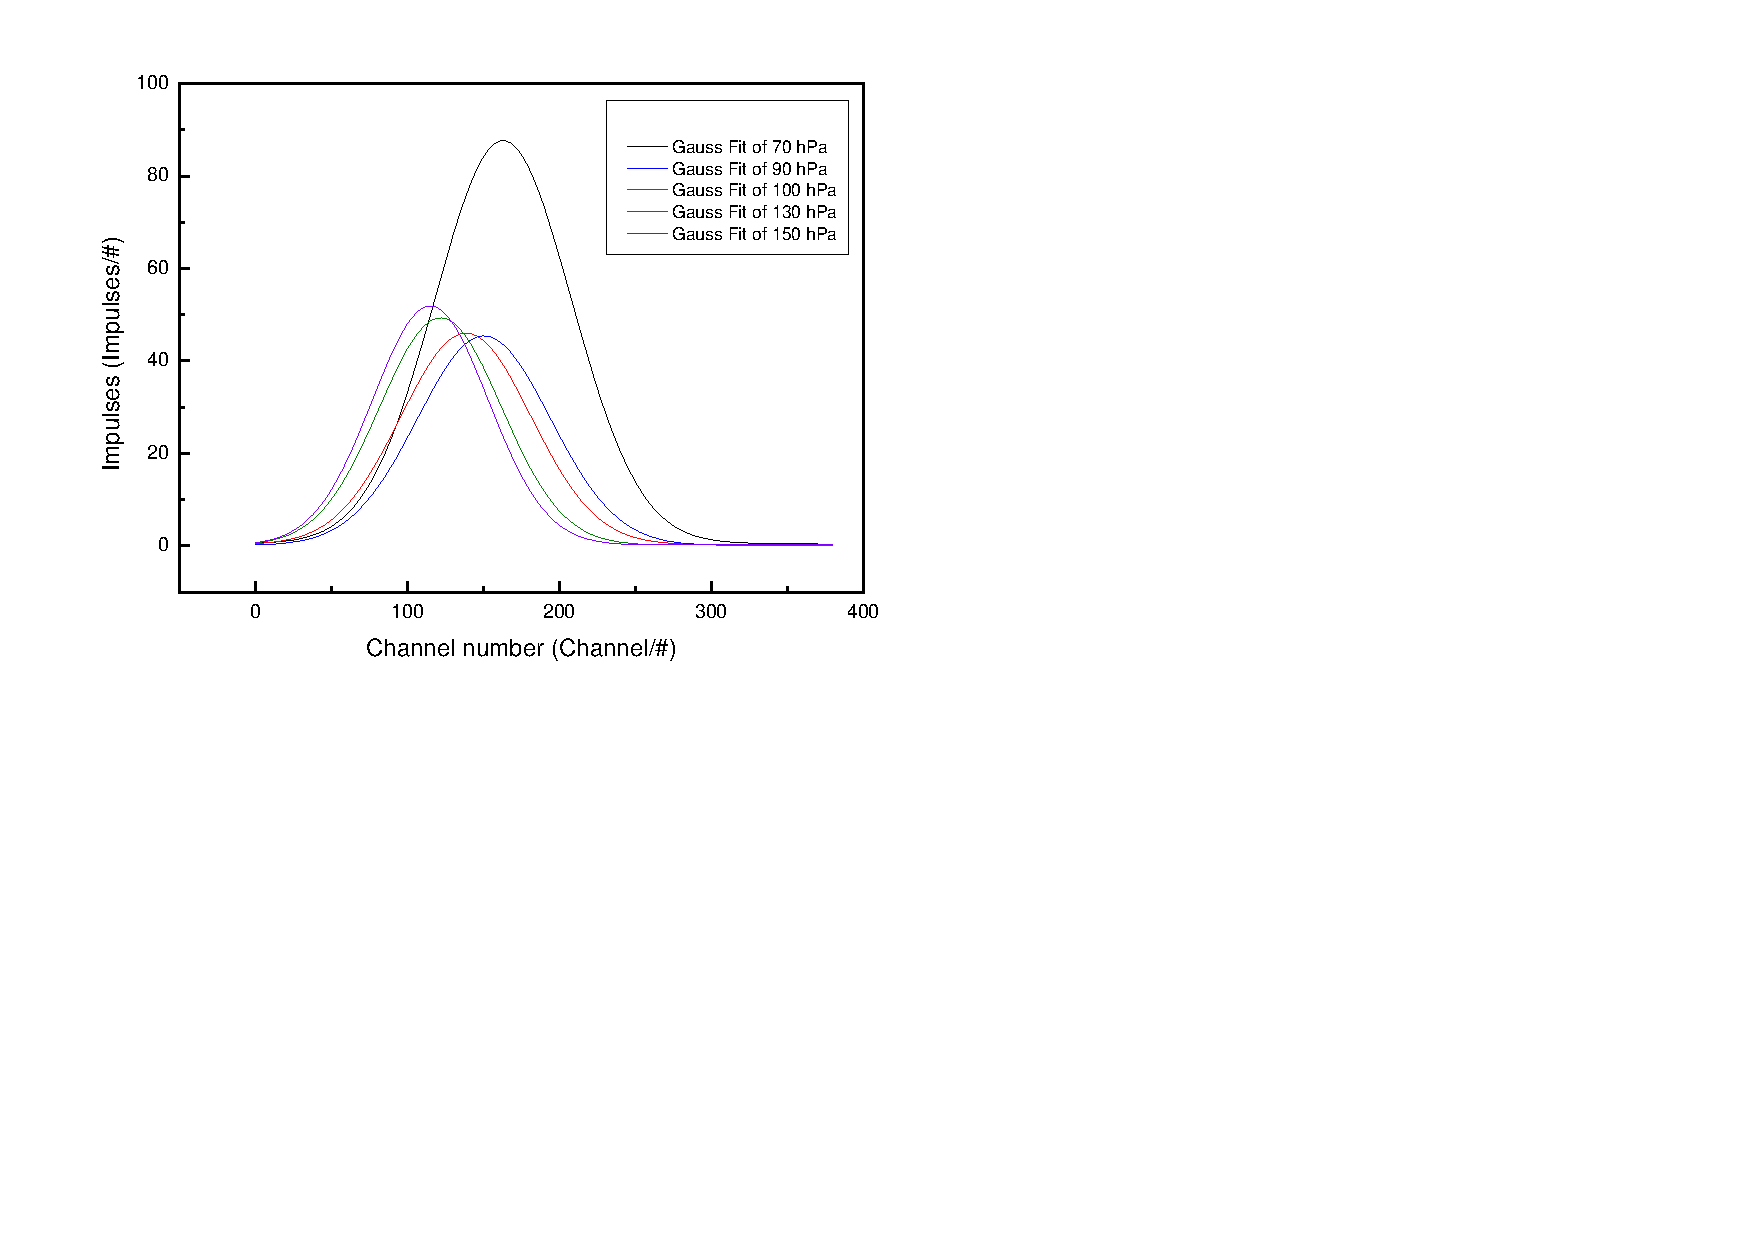
\includegraphics[viewport=1mm 99mm 180mm 200mm, width=9cm, clip=true]{fig5.pdf}
		\caption{압력에 따른 에너지 손실 그래프를 가우시안 함수로 피팅한 것이다.}
		\label{fig:5}
	\end{figure}

	(Fig. 5)에서 검정색 데이터는 70 hPa, 파란색은 90  hPa, 빨간색은 100 hPa, 초록색은 130 hPa, 보라색은 150 hPa이다. 해석하면 데이터의 Peak의 Channel 값, 즉 검출량이 압력이 커질수록 적어짐을 볼 수 있고, 또한 Intensity가 커짐을 볼 수 있다. 70 hPa에서 Intensity가 큰 이유는 event 수를 2배 늘려 실험을 진행했기 때문에, 이러한 경향을 보인다.

	\begin{table}[htb!]
		\label{tab:2}
		\centering
		\caption{압력에 따른 에너지 손실에 관한 표이다.}
		\begin{tabular}{c|ccccc}
			\noalign{\smallskip}\noalign{\smallskip}\hline\hline
			\multirow{2}{*}{Data} &  \multicolumn{5}{c}{Pressure} \\
			\cline{2-6}
				& 70 hPa & 90 hPa & 100 hPa & 130 hPa & 150 hPa \\
			\hline
				Channel No. & 163.28 & 150.68 & 138.84 & 122.13 & 115.39 \\
				Peak Intensity & 87.25 & 45.35 & 45.35 & 49.20 & 51.75 \\
			\hline
			\hline
		\end{tabular}
	\end{table}

	\begin{figure}[htb!]
		\centering
		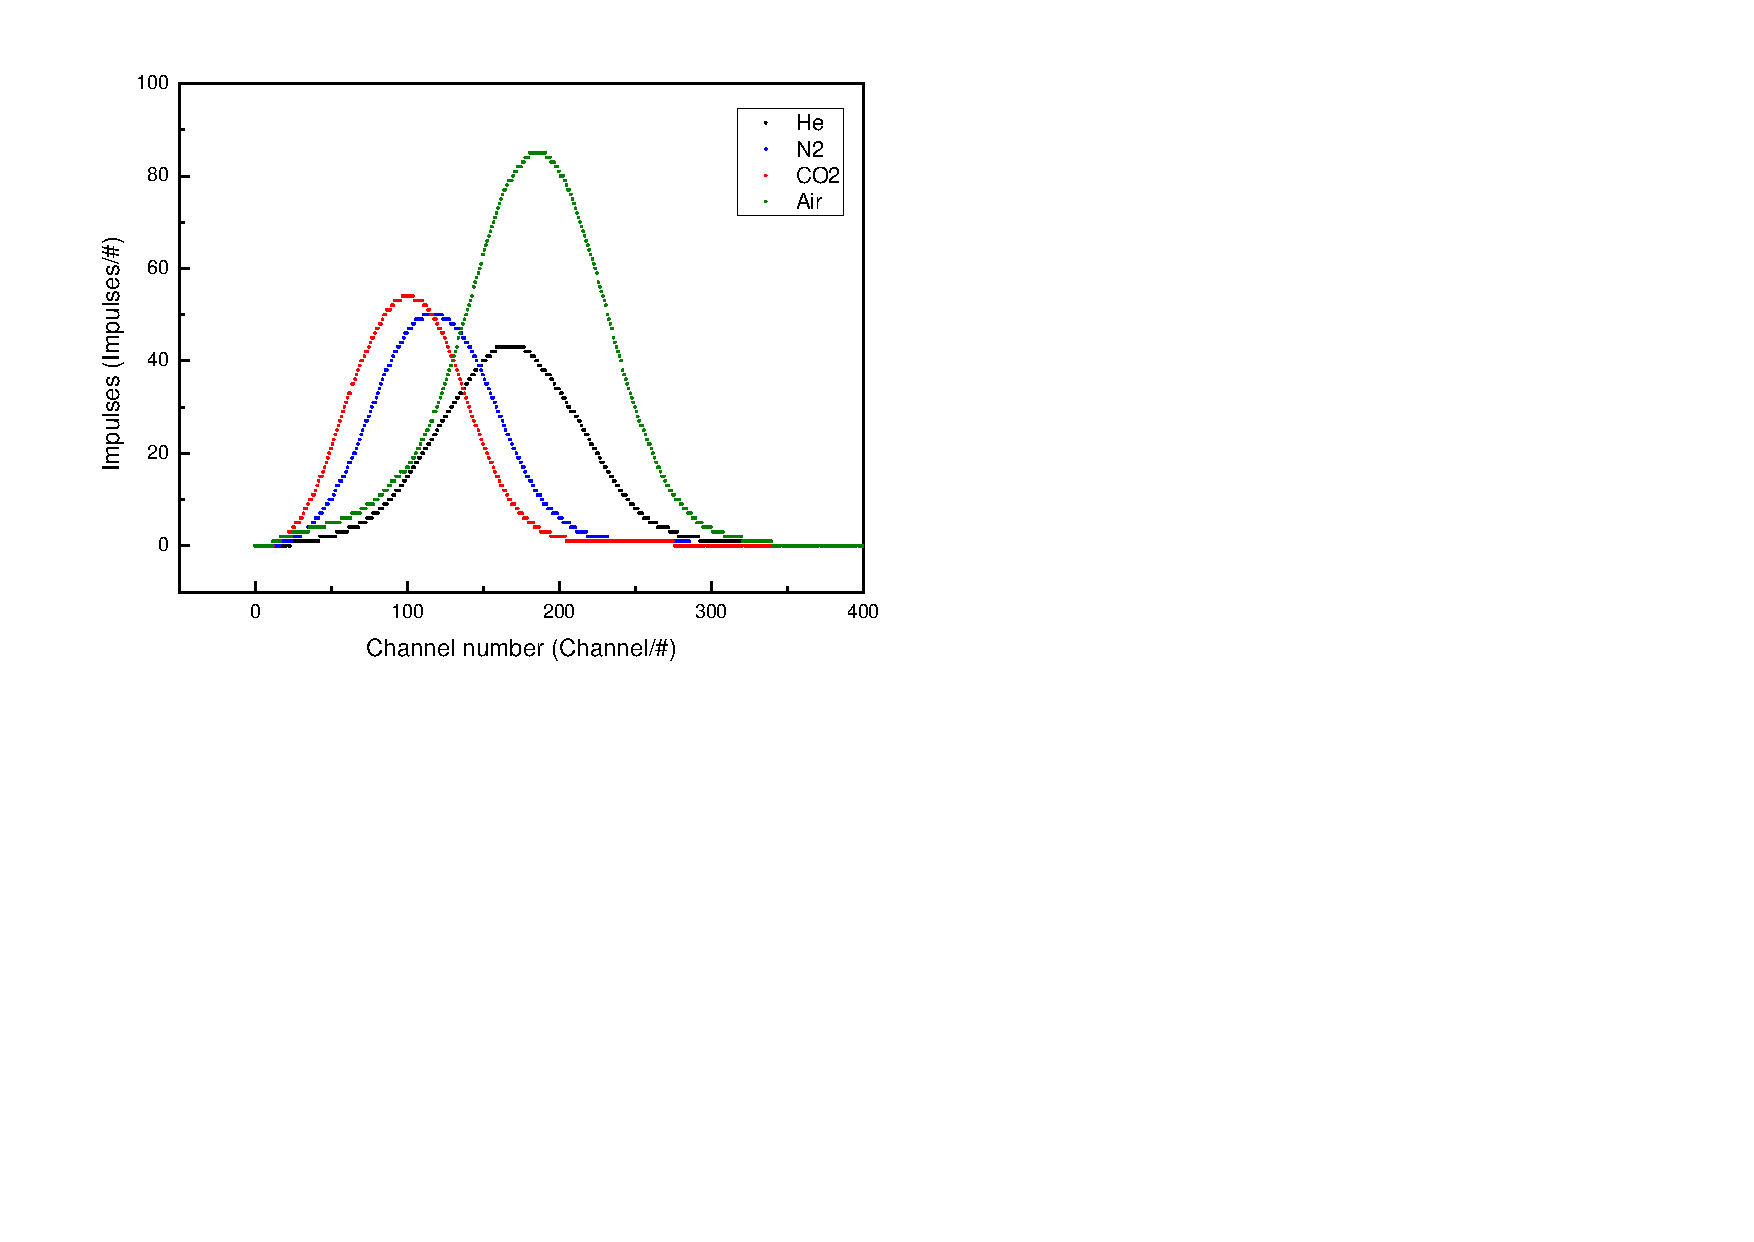
\includegraphics[viewport=1mm 99mm 180mm 200mm, width=9cm, clip=true]{fig6.pdf}
		\caption{기체에 따른 에너지 손실 그래프이다.}
		\label{fig:6}
	\end{figure}

	\begin{figure}[htb!]
		\centering
		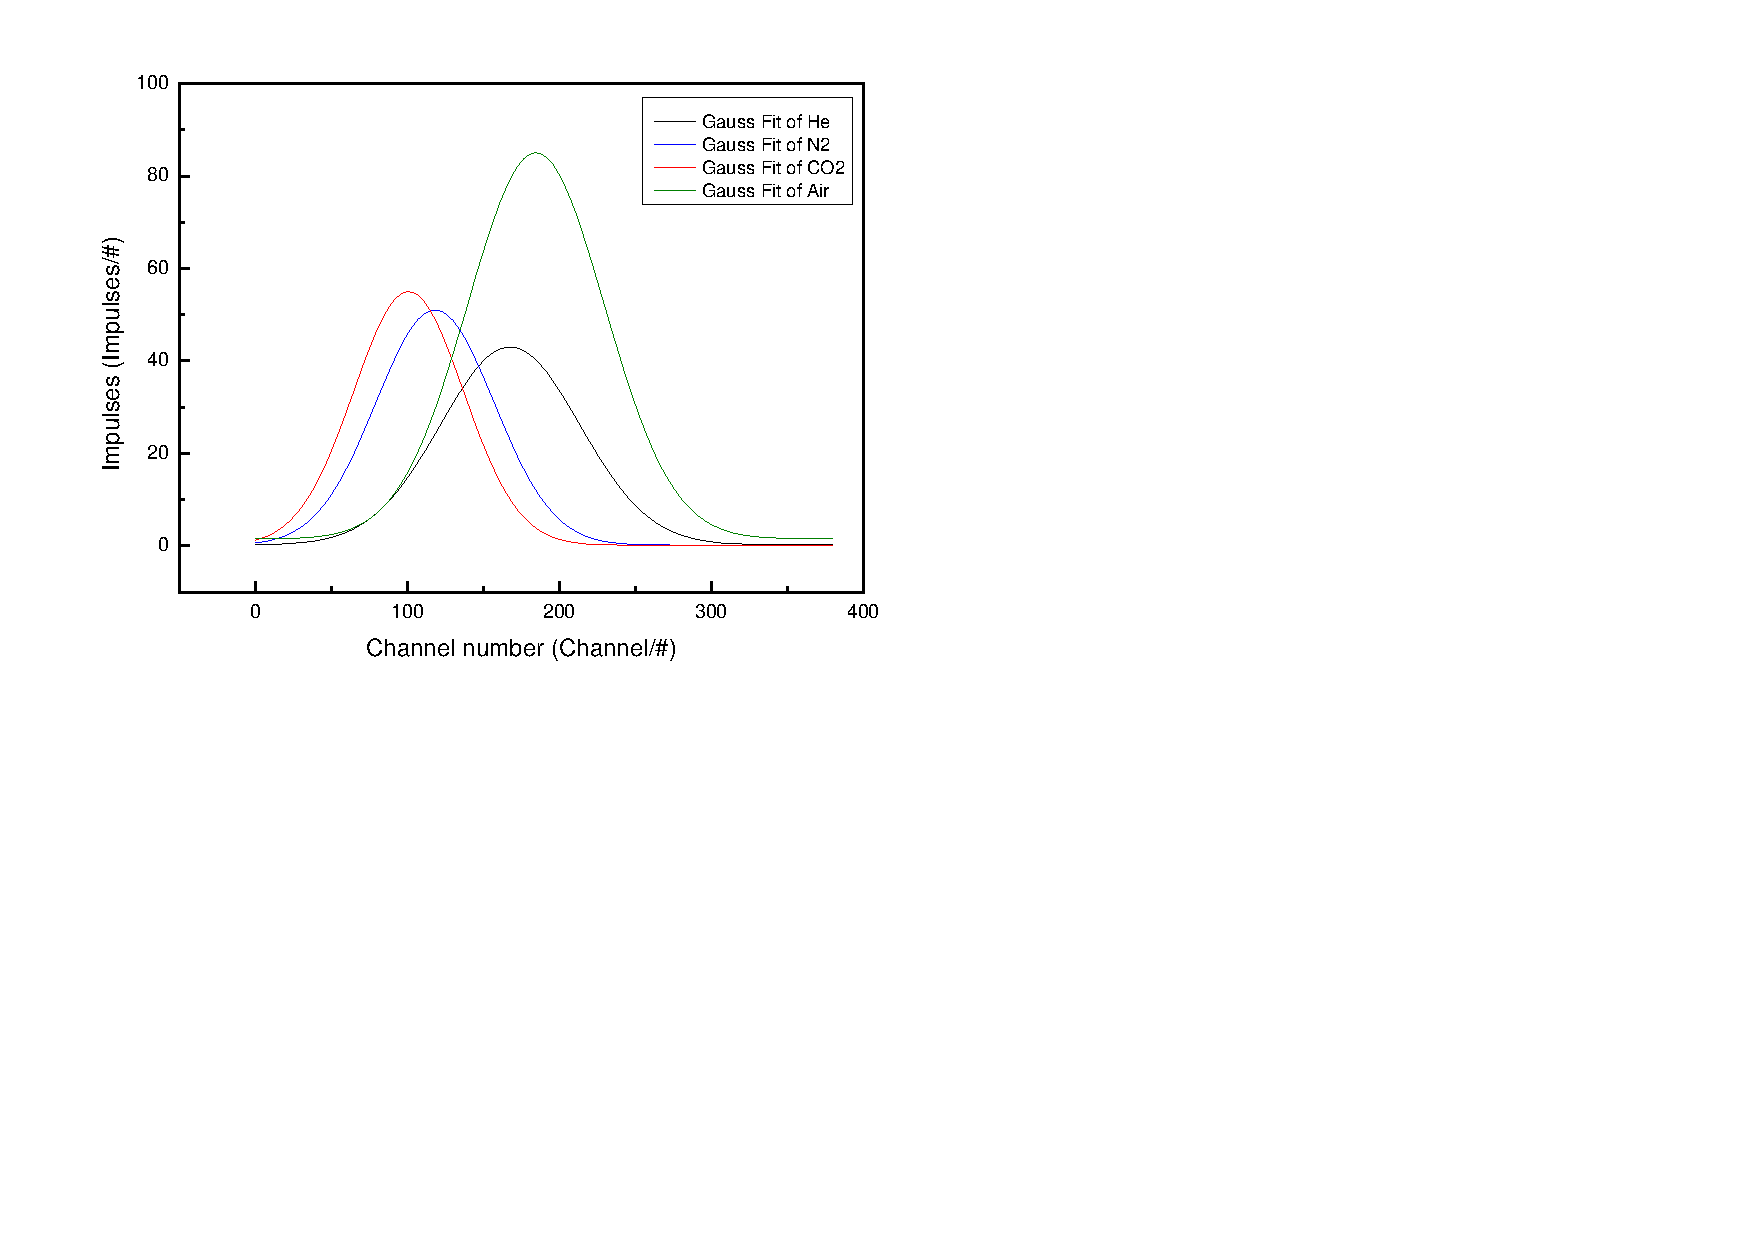
\includegraphics[viewport=1mm 99mm 180mm 200mm, width=9cm, clip=true]{fig7.pdf}
		\caption{기체에 따른 에너지 손실 그래프를 가우시안 함수로 피팅한 것이다.}
		\label{fig:7}
	\end{figure}

	(Fig. 7)에서 검정색 데이터는 He, 파란색은 N$_2$, 빨간색은 CO$_2$, 초록색은 Air이다. 해석하면 데이터의 Peak의 Channel 값, 즉 검출량이 Air, He, N$_2$, CO$_2$의 순으로 적어짐을 볼 수 있고, 또한 Intensity가 커짐을 볼 수 있다. Air에서 Intensity가 큰 이유는 event 수를 2배 늘려 실험을 진행했기 때문에, 이러한 경향을 보인다.


	\begin{table}[htb!]
		\label{tab:3}
		\centering
		\caption{기체에 따른 에너지 손실에 관한 표이다.}
		\begin{tabular}{c|cccc}
			\noalign{\smallskip}\noalign{\smallskip}\hline\hline
			\multirow{2}{*}{Data} &  \multicolumn{4}{c}{Gas} \\
			\cline{2-5}
				& Air & He & N$_2$ & CO$_2$ \\
			\hline
				Channel No. & 167.89 & 118.49 & 101.10 & 184.87 \\
				Peak Intensity & 42.84 & 91.57 & 54.92 & 83.57 \\
			\hline
			\hline
		\end{tabular}
	\end{table}

\subsection{분석}

\begin{align}
	S &= \frac{5000 ~\textrm{ch.} + 50 ~\textrm{ch.}}{5544 ~\textrm{keV}} \\
	&= 0.9921 ~\textrm{Ch./keV} \\
	\varDelta E &= \frac{\varDelta Ch.}{S} \\
	&= 5,040 \\
	\frac{\varDelta E}{Ch.} &= 1.0 ~\textrm{keV/Ch.}
\end{align}

	Channel당 에너지 민감도는 (Eq. 5)와 같다.

	\begin{table}[htb!]
		\label{tab:4}
		\centering
		\caption{}
		\begin{tabular}{c|cccc}
				\noalign{\smallskip}\noalign{\smallskip}\hline\hline
				sort of gas & $k$ & $-\varDelta E/$Ch.\# & $-\varDelta E/$keV & $-\varDelta E/k/$keV \\
			\hline
				He & 2 &  &  &  \\
				N$_2$ & 14 &  &  &   \\
				C0$_2$ & 22 & & & \\
			\hline
			\hline
		\end{tabular}
	\end{table}


%----------------------------------------------------------------------------------------
%	CONCLUSIONS
%----------------------------------------------------------------------------------------

\section{결론}

	알파 입자가 잃게 되는 에너지는 거리에 따라 증가함을 알 수 있었고, 또한 압력에 따라 증가함을 알 수 있었다. 기체에 따라서 에너지 손실값이 달라짐을 알 수 있었고, 그 정도는 헬륨, 질소, 이산화탄소 순이었다.

	압력이 높을 때는 입자의 밀도가 높아 입자에 부딛히는 양이 많아져 에너지를 많이 잃는다고 볼 수 있다. 거리가 큰 경우에는 알파 입자의 속도가 낮아져 입자에 부딛히는 시간이 증가하기에 에너지를 많이 잃는다고 추측할 수 있다. 기체마다 밀도 및 크기가 다르기에 그에 비례하여 결과가 나옴을 추측해 볼 수 있다.

%----------------------------------------------------------------------------------------
%	BIBLIOGRAPHY
%----------------------------------------------------------------------------------------

% \printbibliography % Output the bibliography

%----------------------------------------------------------------------------------------

\end{document}